\documentclass[border=1cm]{standalone}
\usepackage{tikz}
\usepackage{amsmath}

\begin{document}
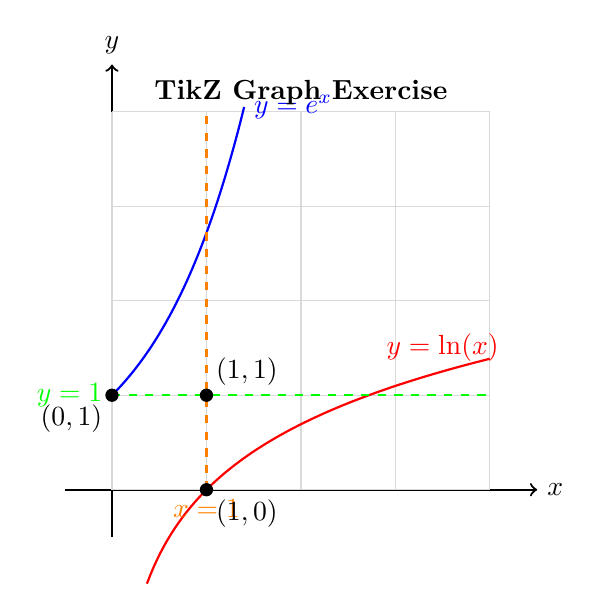
\begin{tikzpicture}[scale=1.2]
    % Draw coordinate system
    \draw[->, thick] (-0.5,0) -- (4.5,0) node[right] {$x$};
    \draw[->, thick] (0,-0.5) -- (0,4.5) node[above] {$y$};
    
    % Draw grid
    \draw[gray!30] (0,0) grid (4,4);
    
    % Draw the curves
    % Exponential function y = e^x
    \draw[blue, thick, domain=0:1.4, samples=100] plot (\x, {exp(\x)});
    \node[blue, right] at (1.4, {exp(1.4)}) {$y = e^x$};
    
    % Natural logarithm y = ln(x)
    \draw[red, thick, domain=0.37:4, samples=100] plot (\x, {ln(\x)});
    \node[red, above] at (3.5, {ln(3.5)}) {$y = \ln(x)$};
    
    % Horizontal line y = 1
    \draw[green, thick, dashed] (0,1) -- (4,1);
    \node[green, left] at (0,1) {$y = 1$};
    
    % Vertical line x = 1
    \draw[orange, thick, dashed] (1,0) -- (1,4);
    \node[orange, below] at (1,0) {$x = 1$};
    
    % Mark intersection points
    \fill[black] (0,1) circle (2pt);
    \fill[black] (1,0) circle (2pt);
    \fill[black] (1,1) circle (2pt);
    
    % Add labels for intersection points
    \node[below left] at (0,1) {$(0,1)$};
    \node[below right] at (1,0) {$(1,0)$};
    \node[above right] at (1,1) {$(1,1)$};
    
    % Add title
    \node[align=center] at (2,4.2) {\textbf{TikZ Graph Exercise}};
\end{tikzpicture}
\end{document}
